\documentclass{beamer}

\usetheme{Madrid}

\usepackage{tikz}
\usetikzlibrary{positioning}
\usetikzlibrary{arrows.meta,positioning}
\usepackage{graphicx}
\usepackage{booktabs}


\title{Chaînes de Markov cachées}
\author{Maxime Delpech et Marius Requillart}
\date{2026}

\begin{document}

\begin{frame}
    \titlepage
\end{frame}

\begin{frame}{Plan}
    \tableofcontents
\end{frame}

\section{Introduction}

\begin{frame}{Définition d'une chaîne de Markov cachée}

\small

\textbf{États cachés.}
Les états cachés sont modélisés par un processus de Markov
\((X_t)_{t\in\mathbb{N}}\) à valeurs dans un ensemble fini
\[
E=\{1,\dots,N\}.
\]
On note \(A=(a_{ij})\) la matrice de transition, avec
\[
a_{ij}=\mathbb{P}(X_{t+1}=j \mid X_t=i).
\]

\vspace{0.2cm}

\textbf{Observations.}
Les observations sont modélisées par un processus
\((Y_t)_{t\in\mathbb{N}}\) à valeurs dans un ensemble \(O\). 
Conditionnellement aux états cachés :
\[
\mathbb{P}(Y_t=y \mid X_t=i)=b_i(y),
\]
où \(B=(b_i(y))\) est la matrice, ou famille, d'émission.

\vspace{0.2cm}

\textbf{Modèle HMM.}
Un modèle de chaîne de Markov cachée est défini par le triplet
\[
(A,B,\pi),
\]
où \(A\) est la matrice de transition, \(B\) la loi d'émission et
\(\pi\) la distribution initiale.

\end{frame}



\begin{frame}{Exemple global d'une chaîne de Markov cachée}

\large

\[
E=\{C,V\},
\qquad
\pi_0=(0.5,0.5)
\]

\vspace{0.4cm}

\[
A=
\begin{pmatrix}
0.9 & 0.1 \\
0.2 & 0.8
\end{pmatrix}
\]

\vspace{0.3cm}

\[
a_{ij}=\mathbb{P}(X_{t+1}=j\mid X_t=i)
\]

\vspace{0.4cm}

\[
B=
\begin{cases}
\mathcal{L}(Y_t\mid X_t=C)\sim \mathcal{N}(\mu_C,\sigma_C^2),\\
\mathcal{L}(Y_t\mid X_t=V)\sim \mathcal{N}(\mu_V,\sigma_V^2).
\end{cases}
\]

\end{frame}


\begin{frame}{Structure du modèle HMM}

\centering

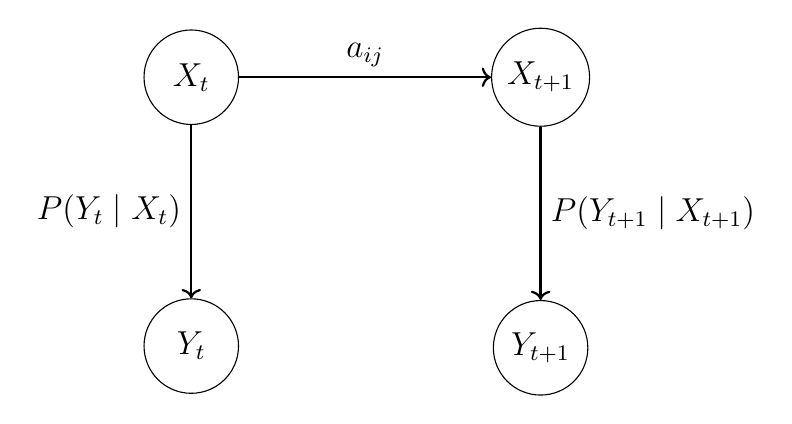
\begin{tikzpicture}[
    node distance=2.2cm,
    state/.style={draw, circle, minimum size=1.2cm, font=\large},
    arrow/.style={->, thick},
    labelnode/.style={draw=none, font=\large}
]

\node[state] (X1) {$X_t$};
\node[state, right=3.2cm of X1] (X2) {$X_{t+1}$};

\node[state, below=2.2cm of X1] (Y1) {$Y_t$};
\node[state, below=2.2cm of X2] (Y2) {$Y_{t+1}$};

\draw[arrow] (X1) -- node[midway, above, labelnode] {$a_{ij}$} (X2);

\draw[arrow] (X1) -- 
node[midway, left, labelnode] {$\mathbb{P}(Y_t\mid X_t)$} 
(Y1);

\draw[arrow] (X2) -- 
node[midway, right, labelnode] {$\mathbb{P}(Y_{t+1}\mid X_{t+1})$} 
(Y2);

\end{tikzpicture}

\vspace{0.4cm}

\small
Les états cachés évoluent selon \(A\), et chaque observation est générée conditionnellement à l'état courant.

\end{frame}


\begin{frame}{Les observations ne sont pas markoviennes}

\small

\textbf{Propriété.}
Dans un HMM non dégénéré, le processus d'observations \((Y_t)_t\) n'est pas un processus de Markov, même si les états cachés \((X_t)_t\) le sont.

\vspace{0.35cm}
On a : 

\[
\mathbb{P}(Y_{n+1}\mid Y_1,\dots,Y_n)
=
\sum_{i=1}^{K}
\mathbb{P}(Y_{n+1}\mid X_{n+1}=i)
\mathbb{P}(X_{n+1}=i\mid Y_1,\dots,Y_n)
\]

Or,

\[
\mathbb{P}(X_{n+1}=i\mid Y_1,\dots,Y_n)
=
\sum_{j=1}^{K}
\mathbb{P}(X_{n+1}=i,X_n=j\mid Y_1,\dots,Y_n)
\]

Et

\[
\mathbb{P}(X_{n+1}=i\mid Y_1,\dots,Y_n)
=
\sum_{j=1}^{K}
a_{ji}\mathbb{P}(X_n=j\mid Y_1,\dots,Y_n)
\]

\end{frame}

\begin{frame}{Dépendance au passé observé}

\scriptsize

\begin{align*}
\mathbb{P}(X_n=j\mid Y_1,\dots,Y_n)
&=
\frac{
\mathbb{P}(Y_n\mid X_n=j,Y_1,\dots,Y_{n-1})
\mathbb{P}(X_n=j,Y_1,\dots,Y_{n-1})
}{
\mathbb{P}(Y_1,\dots,Y_n)
}
\\[0.45cm]
\mathbb{P}(X_n=j\mid Y_1,\dots,Y_n)
&=
\frac{
\mathbb{P}(Y_n\mid X_n=j)
\mathbb{P}(X_n=j\mid Y_1,\dots,Y_{n-1})
}{
\mathbb{P}(Y_n\mid Y_1,\dots,Y_{n-1})
}.
\end{align*}

\vspace{0.25cm}

\[
\begin{aligned}
\mathbb{P}(Y_{n+1}\mid Y_1,\dots,Y_n)
&=
\sum_{i=1}^{K}\sum_{j=1}^{K}
a_{ji}
\frac{
\mathbb{P}(Y_{n+1}\mid X_{n+1}=i)
\mathbb{P}(Y_n\mid X_n=j)
}{
\mathbb{P}(Y_n\mid Y_1,\dots,Y_{n-1})
}
\\[0.2cm]
&\qquad\qquad\qquad\qquad\times
\mathbb{P}(X_n=j\mid Y_1,\dots,Y_{n-1}).
\end{aligned}
\]

\vspace{0.25cm}
Ainsi, on remarque bien que 
\[
\mathbb{P}(Y_{n+1}\mid Y_1,\dots,Y_n)
\neq
\mathbb{P}(Y_{n+1}\mid Y_n).
\]

\end{frame}

\begin{frame}{Algorithme Forward}

\small

La vraisemblance de la séquence observée est :
\[
\mathbb{P}(Y)
=
\sum_X \mathbb{P}(Y,X)
=
\sum_X \mathbb{P}(Y\mid X)\mathbb{P}(X).
\]

\vspace{0.25cm}

\begin{block}{Principe}
On définit
\[
\alpha_t(i)=\mathbb{P}(y_1,\dots,y_t,X_t=i).
\]


\vspace{0.15cm}

\textbf{Initialisation}
\[
\alpha_1(i)=\pi_i b_i(y_1),
\qquad i=1,\dots,N.
\]

\textbf{Récursion}
\[
\alpha_t(j)
=
b_j(y_t)\sum_{i=1}^{N}\alpha_{t-1}(i)a_{ij},
\qquad t=2,\dots,T.
\]

\textbf{Terminaison}
\[
\mathbb{P}(Y)=\sum_{i=1}^{N}\alpha_T(i).
\]
\end{block}

\end{frame}


\begin{frame}{Algorithme de Viterbi}

\scriptsize

On estime le chemin le plus problable avec : 
\[
\delta_t(i)
=
\max_{X_1,\dots,X_{t-1}}
\mathbb{P}(X_1,\dots,X_t=i,y_1,\dots,y_t\mid \lambda)
\]

\[
\delta_{t+1}(j)
=
\left[
\max_{1\leq i\leq N}
\delta_t(i)a_{ij}
\right]
b_j(y_{t+1})
\]

\vspace{0.15cm}

\centering
\resizebox{0.95\textwidth}{!}{%
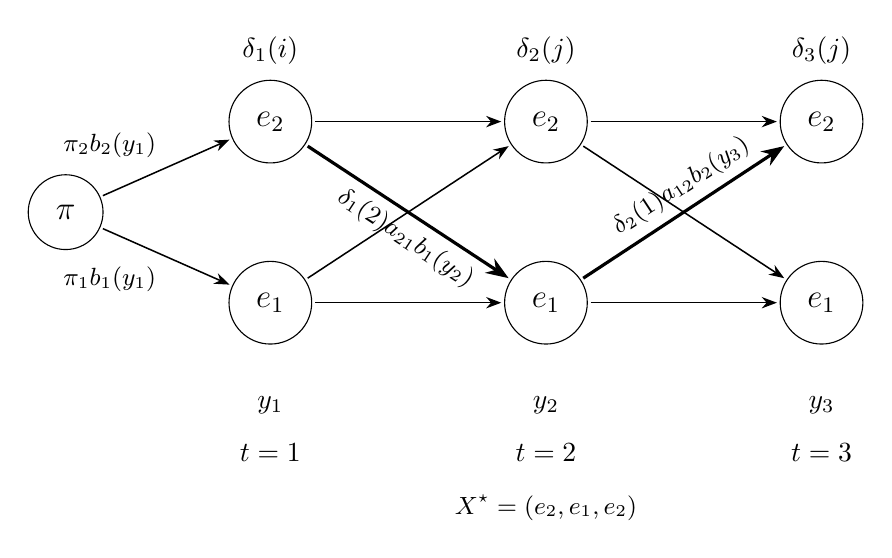
\begin{tikzpicture}[
    >=Stealth,
    etat/.style={
        circle,
        draw,
        minimum size=1.05cm,
        inner sep=0pt,
        font=\large
    },
    init/.style={
        circle,
        draw,
        minimum size=0.95cm,
        inner sep=0pt,
        font=\large
    },
    fleche/.style={
        ->,
        line width=0.55pt,
        shorten >=1pt,
        shorten <=1pt
    },
    flechemax/.style={
        ->,
        line width=1.15pt,
        shorten >=1pt,
        shorten <=1pt
    },
    formule/.style={
        font=\small
    }
]

\node[init] (pi) at (0,0) {$\pi$};

\node[etat] (e21) at (2.6,1.15) {$e_2$};
\node[etat] (e11) at (2.6,-1.15) {$e_1$};

\node[etat] (e22) at (6.1,1.15) {$e_2$};
\node[etat] (e12) at (6.1,-1.15) {$e_1$};

\node[etat] (e23) at (9.6,1.15) {$e_2$};
\node[etat] (e13) at (9.6,-1.15) {$e_1$};

\node at (2.6,-2.45) {$y_1$};
\node at (6.1,-2.45) {$y_2$};
\node at (9.6,-2.45) {$y_3$};

\draw[fleche] (pi) -- node[above left, formule] {$\pi_2 b_2(y_1)$} (e21);
\draw[fleche] (pi) -- node[below left, formule] {$\pi_1 b_1(y_1)$} (e11);

\draw[fleche] (e21) -- (e22);
\draw[flechemax] (e21) -- node[pos=0.55, below, sloped, formule]
{$\delta_1(2)a_{21}b_1(y_2)$} (e12);
\draw[fleche] (e11) -- (e22);
\draw[fleche] (e11) -- (e12);

\draw[fleche] (e22) -- (e23);
\draw[fleche] (e22) -- (e13);
\draw[flechemax] (e12) -- node[pos=0.55, above, sloped, formule]
{$\delta_2(1)a_{12}b_2(y_3)$} (e23);
\draw[fleche] (e12) -- (e13);

\node at (2.6,2.05) {\(\delta_1(i)\)};
\node at (6.1,2.05) {\(\delta_2(j)\)};
\node at (9.6,2.05) {\(\delta_3(j)\)};

\node at (2.6,-3.05) {\(t=1\)};
\node at (6.1,-3.05) {\(t=2\)};
\node at (9.6,-3.05) {\(t=3\)};

\node[formule, align=center] at (6.1,-3.75)
{\(\displaystyle X^\star=(e_2,e_1,e_2)\)};

\end{tikzpicture}
}

\vspace{0.1cm}

{\scriptsize Treillis de l'algorithme de Viterbi}

\end{frame}


\begin{frame}{Algorithme de Baum--Welch : étape E}

\scriptsize

Baum--Welch est un algorithme EM : à partir d'un modèle courant
\[
\lambda^{(k)}=(\pi^{(k)},A^{(k)},B^{(k)}),
\]
on estime les états cachés, puis on met à jour les paramètres.

\vspace{0.25cm}

\textbf{Probabilité d'être dans l'état \(i\) au temps \(t\) :}
\[
\gamma_t(i)
=
\mathbb{P}(X_t=i\mid Y,\lambda^{(k)})
=
\frac{\alpha_t(i)\beta_t(i)}
{\sum_{\ell=1}^{N}\alpha_t(\ell)\beta_t(\ell)}.
\]

\vspace{0.25cm}

\textbf{Probabilité de transition \(i\to j\) entre \(t\) et \(t+1\) :}
\[
\xi_t(i,j)
=
\mathbb{P}(X_t=i,X_{t+1}=j\mid Y,\lambda^{(k)}).
\]

\[
\xi_t(i,j)
=
\frac{
\alpha_t(i)a_{ij}^{(k)}b_j^{(k)}(y_{t+1})\beta_{t+1}(j)
}{
\sum_{r=1}^{N}\sum_{s=1}^{N}
\alpha_t(r)a_{rs}^{(k)}b_s^{(k)}(y_{t+1})\beta_{t+1}(s)
}.
\]

\vspace{0.2cm}

\[
\gamma_t(i)
\quad \text{et} \quad
\xi_t(i,j)
\]
donnent les nombres moyens de visites des états et de transitions.

\end{frame}

\begin{frame}{Algorithme de Baum--Welch : étape M}

\scriptsize

Une fois \(\gamma_t(i)\) et \(\xi_t(i,j)\) calculés, on met à jour les paramètres.

\vspace{0.25cm}

\textbf{Distribution initiale :}
\[
\pi_i^{(k+1)}=\gamma_1(i).
\]

\vspace{0.25cm}

\textbf{Matrice de transition :}
\[
a_{ij}^{(k+1)}
=
\frac{
\sum_{t=1}^{T-1}\xi_t(i,j)
}{
\sum_{t=1}^{T-1}\gamma_t(i)
}.
\]

\vspace{0.25cm}

\textbf{Émissions discrètes :}
\[
b_j^{(k+1)}(y)
=
\frac{
\sum_{t=1}^{T}\gamma_t(j)\mathbf{1}_{\{Y_t=y\}}
}{
\sum_{t=1}^{T}\gamma_t(j)
}.
\]

\vspace{0.25cm}

\textbf{Émissions gaussiennes :}
\[
\mu_j^{(k+1)}
=
\frac{
\sum_{t=1}^{T}\gamma_t(j)Y_t
}{
\sum_{t=1}^{T}\gamma_t(j)
},
\qquad
(\sigma_j^2)^{(k+1)}
=
\frac{
\sum_{t=1}^{T}\gamma_t(j)(Y_t-\mu_j^{(k+1)})^2
}{
\sum_{t=1}^{T}\gamma_t(j)
}.
\]

\vspace{0.2cm}

On répète ces étapes jusqu'à stabilisation de
\[
\ell^{(k)}=\log \mathbb{P}(Y\mid \lambda^{(k)}).
\]

\end{frame}


\begin{frame}{Évaluation de l'algorithme Forward}

\small

L'algorithme Forward permet d'évaluer la qualité du modèle à partir de la vraisemblance :
\[
\ell(\lambda)=\log \mathbb{P}(Y_{1:T}\mid \lambda).
\]

\vspace{0.25cm}

\textbf{Critères utilisés :}

\begin{itemize}
    \item \textbf{Log-vraisemblance moyenne}
    \[
    \bar{\ell}(\lambda)=\frac{1}{T}\ell(\lambda)
    \]

    \item \textbf{Critères pénalisés}
    \[
    AIC=-2\ell(\lambda)+2p,
    \qquad
    BIC=-2\ell(\lambda)+p\log(T)
    \]

    \item \textbf{Validation hors échantillon}
    \[
    NLPD_{\text{test}}
    =
    -\frac{1}{T_{\text{test}}}
    \log \mathbb{P}(Y_{\text{test}}\mid \widehat{\lambda}_{\text{train}})
    \]
\end{itemize}

\vspace{0.1cm}

\scriptsize
Une bonne performance Forward correspond à une log-vraisemblance élevée, des critères AIC/BIC faibles, et une NLPD stable sur les données de test.

\end{frame}


\begin{frame}{Évaluation de l'algorithme de Viterbi}

\small

Viterbi estime la trajectoire cachée la plus probable :
\[
\widehat X_{1:T}^{\,V}
\in
\arg\max_{x_{1:T}}
\mathbb{P}(X_{1:T}=x_{1:T}\mid Y_{1:T},\widehat{\lambda}).
\]

\vspace{0.25cm}

\textbf{Critères utilisés :}

\begin{itemize}
    \item \textbf{Interprétation des régimes} : vérifier si les états détectés correspondent à des comportements observables distincts.

    \item \textbf{Persistance des régimes} :
    \[
    \text{taux de changement}
    =
    \frac{1}{T-1}
    \sum_{t=1}^{T-1}
    \mathbf{1}_{\{\widehat X_t^V\neq \widehat X_{t+1}^V\}}.
    \]

    \item \textbf{Comparaison avec le posterior decoding et le decoding local}
    \[
    D_{VP}
    =
    \frac{1}{T}
    \sum_{t=1}^{T}
    \mathbf{1}_{\{\widehat X_t^V\neq \widehat X_t^P\}}.
    \]
\end{itemize}

\vspace{0.1cm}

\scriptsize
Un bon décodage est cohérent temporellement, interprétable, et proche du posterior decoding lorsque l'incertitude sur les états est faible.

\end{frame}


\begin{frame}{Évaluation de l'algorithme de Baum--Welch}

\small

Baum--Welch estime les paramètres du modèle :
\[
\widehat{\lambda}
=
(\widehat{\pi},\widehat{A},\widehat{B})
\in
\arg\max_{\lambda}
\mathbb{P}(Y_{1:T}\mid \lambda).
\]

\vspace{0.25cm}

\textbf{Critères utilisés :}

\begin{itemize}
    \item \textbf{Convergence de la log-vraisemblance}
    \[
    \Delta_k=\ell^{(k)}-\ell^{(k-1)},
    \qquad
    r_k=
    \frac{\Delta_k}{1+|\ell^{(k-1)}|}.
    \]

    \item \textbf{Stabilité selon l'initialisation}
    \[
    D_A=
    \frac{1}{N}\sum_i
    \frac{1}{2}\sum_j
    |\widehat a_{ij}^{(a)}-\widehat a_{ij}^{(b)}|.
    \]

    \item \textbf{Interprétation des régimes} : les états estimés doivent correspondre à des comportements distincts.

    \item \textbf{Validation hors échantillon}
    \[
    NLPD_{\text{test}}
    =
    -\frac{1}{T_{\text{test}}}
    \log \mathbb{P}(Y_{\text{test}}\mid \widehat{\lambda}_{\text{train}}).
    \]
\end{itemize}

\end{frame}


\begin{frame}{Simulation d'une chaîne de Markov cachée}

\small

On simule un HMM à trois états cachés :
\[
S=\{\text{soleil},\text{nuageux},\text{pluie}\}
\]
et deux observations possibles :
\[
O=\{\text{parapluie},\text{pas parapluie}\}.
\]

\vspace{0.25cm}

\[
\pi=
\begin{pmatrix}
0.5 & 0.3 & 0.2
\end{pmatrix}
\]

\[
A=
\begin{pmatrix}
0.7 & 0.295 & 0.005 \\
0.3 & 0.4 & 0.3 \\
0.005 & 0.395 & 0.6
\end{pmatrix}
\qquad
B=
\begin{pmatrix}
0.1 & 0.9 \\
0.4 & 0.6 \\
0.9 & 0.1
\end{pmatrix}
\]

\vspace{0.2cm}

La trajectoire simulée contient \(T=1001\) observations, avec les vrais états cachés connus.

\end{frame}



\begin{frame}{Résultats bruts des algorithmes sur la simulation}

\scriptsize

\textbf{Forward}
\[
\log \mathbb{P}(Y_{1:T}\mid\lambda)
=
-639.814329.
\]

\vspace{0.15cm}

\textbf{Viterbi}

\begin{center}
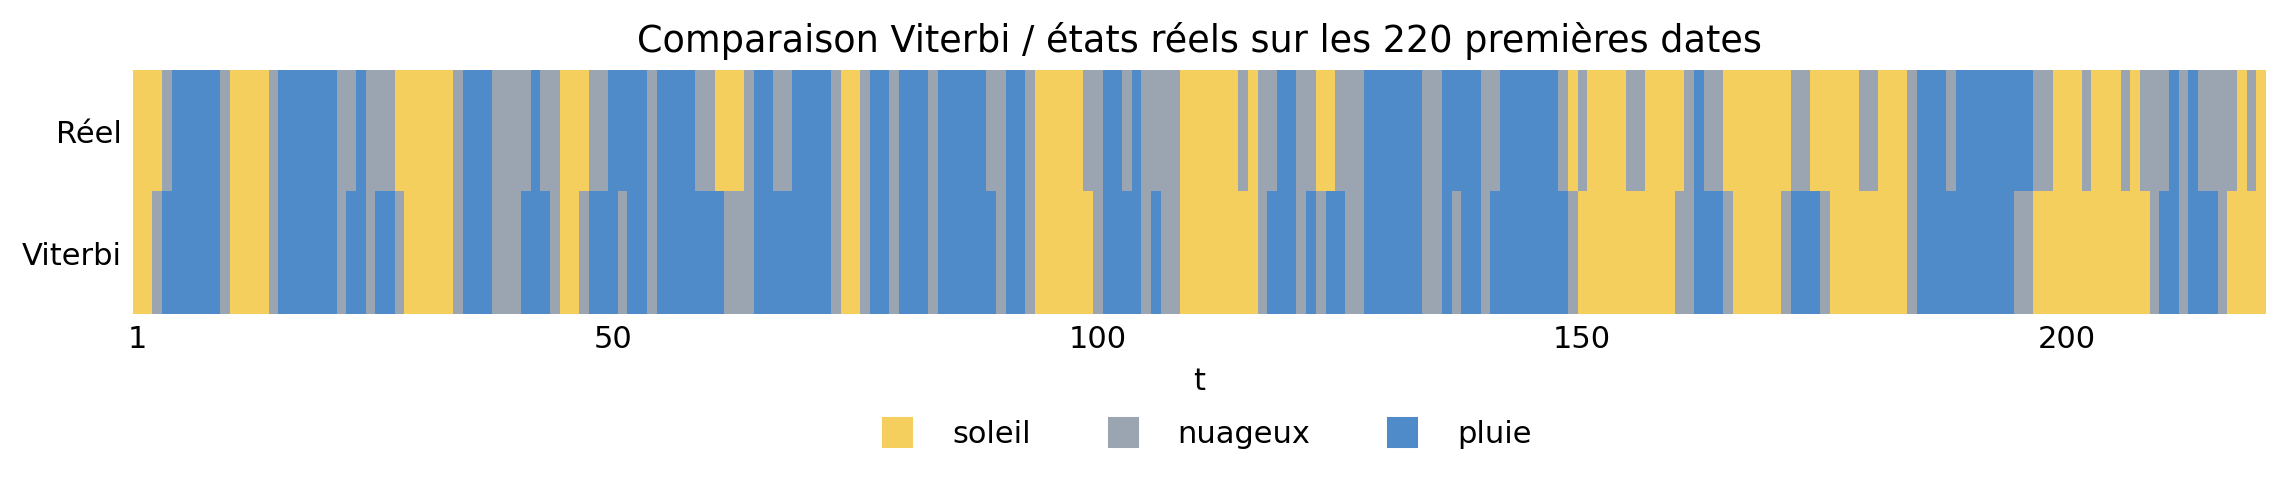
\includegraphics[width=0.78\linewidth]{Test/viterbi_vs_reel_220.png}
\end{center}

\vspace{0.1cm}

\textbf{Baum--Welch}

\[
\widehat A=
\begin{pmatrix}
0.7026 & 0.2956 & 0.0018 \\
0.2720 & 0.5963 & 0.1316 \\
0.1804 & 0.2172 & 0.6024
\end{pmatrix}
\qquad
\widehat B=
\begin{pmatrix}
0.1070 & 0.8930 \\
0.5702 & 0.4298 \\
0.9895 & 0.0105
\end{pmatrix}
\]

\end{frame}

\begin{frame}{Analyse Forward sur la simulation}

\tiny
\centering

\vspace{-0.2cm}

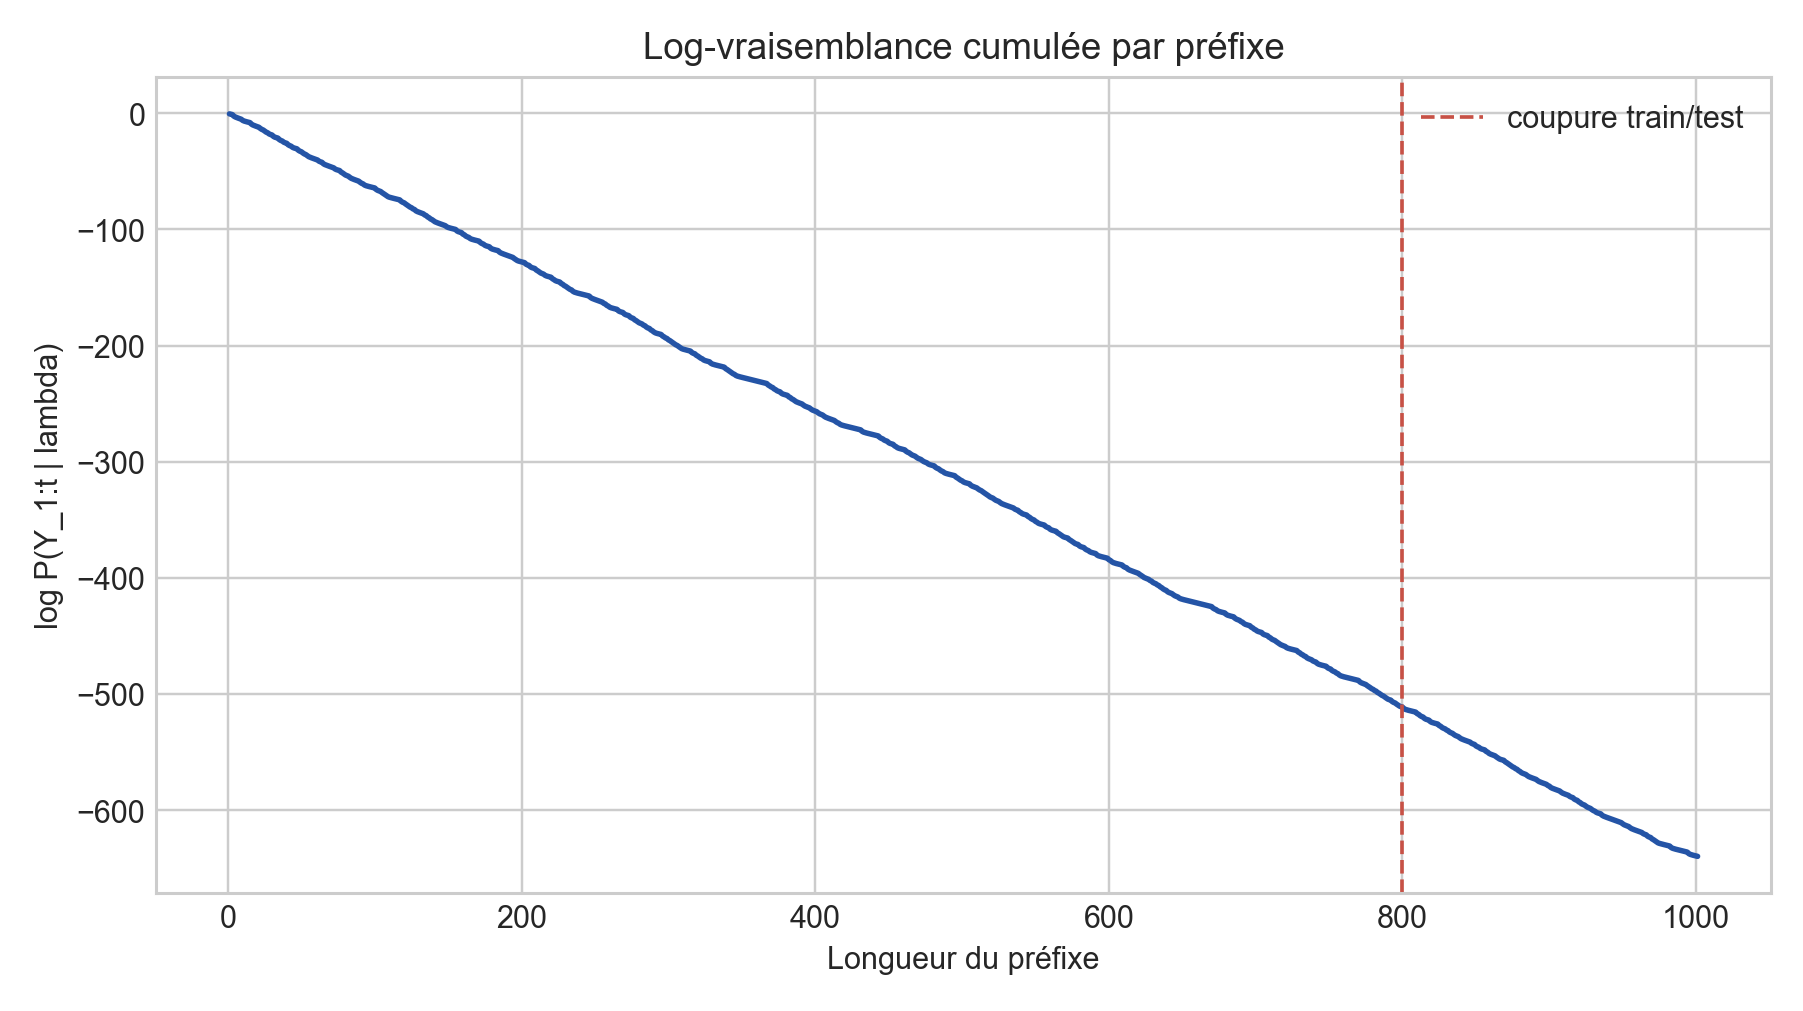
\includegraphics[width=0.48\linewidth]{Test/prefix_log_likelihood.png}

\vspace{-0.1cm}

\textbf{Comparaison de modèles}

\vspace{0.1cm}

\resizebox{0.86\linewidth}{!}{
\begin{tabular}{lrrrrr}
\toprule
Modèle & log-vrais. & log-vrais./obs. & NLPD & AIC & BIC \\
\midrule
Simulation & -639.814329 & -0.639175 & 0.639175 & 1301.628658 & 1355.624961 \\
Transitions unif. & -689.395632 & -0.688707 & 0.688707 & 1400.791264 & 1454.787566 \\
Émissions unif. & -693.840328 & -0.693147 & 0.693147 & 1409.680655 & 1463.676958 \\
Modèle unif. & -693.840328 & -0.693147 & 0.693147 & 1409.680655 & 1463.676958 \\
\bottomrule
\end{tabular}
}

\vspace{0.1cm}

\textbf{Validation hors échantillon}

\vspace{0.1cm}

\resizebox{0.80\linewidth}{!}{
\begin{tabular}{lrrrr}
\toprule
Segment & \(T\) & log-vrais. & log-vrais./obs. & NLPD \\
\midrule
Apprentissage & 800 & -511.319586 & -0.639149 & 0.639149 \\
Test cond. & 201 & -128.494743 & -0.639277 & 0.639277 \\
Test indép. & 201 & -128.462530 & -0.639117 & 0.639117 \\
\bottomrule
\end{tabular}
}

\end{frame}


\begin{frame}{Analyse Viterbi sur la simulation}

\tiny
\centering

\begin{columns}[T]

\begin{column}{0.50\textwidth}
\centering
\textbf{Persistance des séquences}

\vspace{0.05cm}

\resizebox{\linewidth}{!}{
\begin{tabular}{lrrrrr}
\toprule
Séquence & Chang. & Taux & Runs & Moy. & Max \\
\midrule
Viterbi & 326 & 32.60\% & 327 & 3.06 & 28 \\
Posterior decoding & 390 & 39.00\% & 391 & 2.56 & 21 \\
Décodage local & 358 & 35.80\% & 359 & 2.79 & 23 \\
\bottomrule
\end{tabular}
}
\end{column}

\begin{column}{0.50\textwidth}
\centering
\textbf{Viterbi vs posterior decoding}

\vspace{0.05cm}

\resizebox{\linewidth}{!}{
\begin{tabular}{lr}
\toprule
Critère & Valeur \\
\midrule
\(D_{VP}\) & 8.39\% \\
Désaccord Viterbi / décodage local & 24.48\% \\
Proba post. moyenne Viterbi & 66.04\% \\
Proba post. médiane Viterbi & 67.99\% \\
Marge post. moyenne & 38.33\% \\
Marge post. médiane & 42.12\% \\
\bottomrule
\end{tabular}
}
\end{column}

\end{columns}

\vspace{0.25cm}

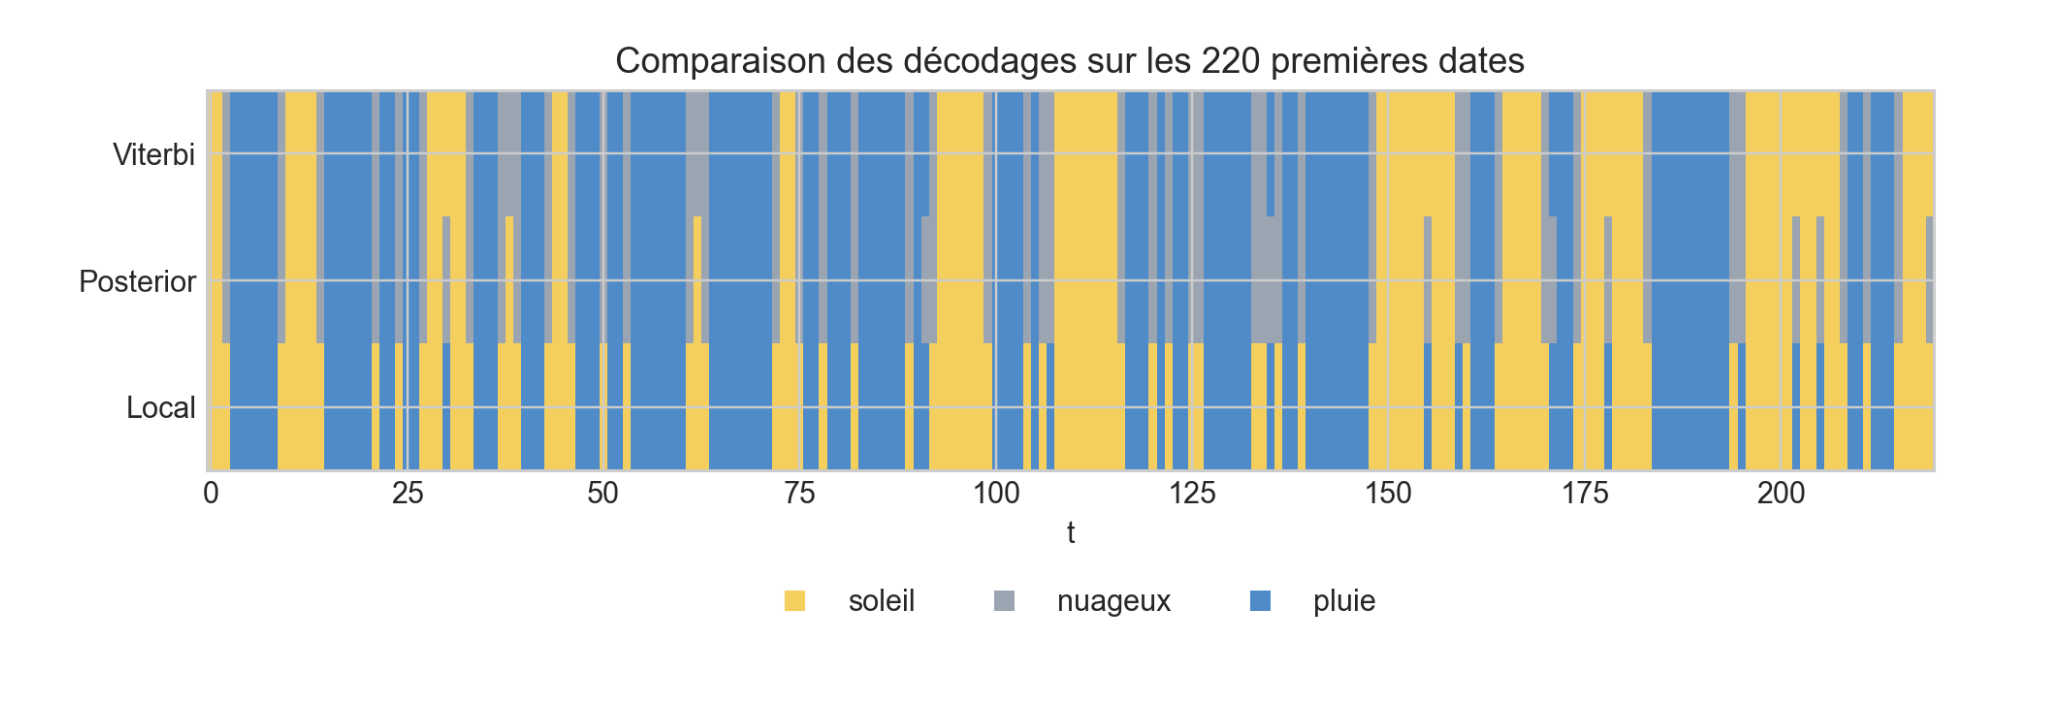
\includegraphics[width=0.78\linewidth]{Test/comparaison_visuelle_Viterbi.png}

\vspace{0.05cm}

{\tiny Comparaison visuelle entre Viterbi, posterior decoding et décodage local.}

\end{frame}


\begin{frame}{Analyse Baum--Welch sur la simulation}

\tiny
\centering

\begin{columns}[T]

\begin{column}{0.50\textwidth}
\centering
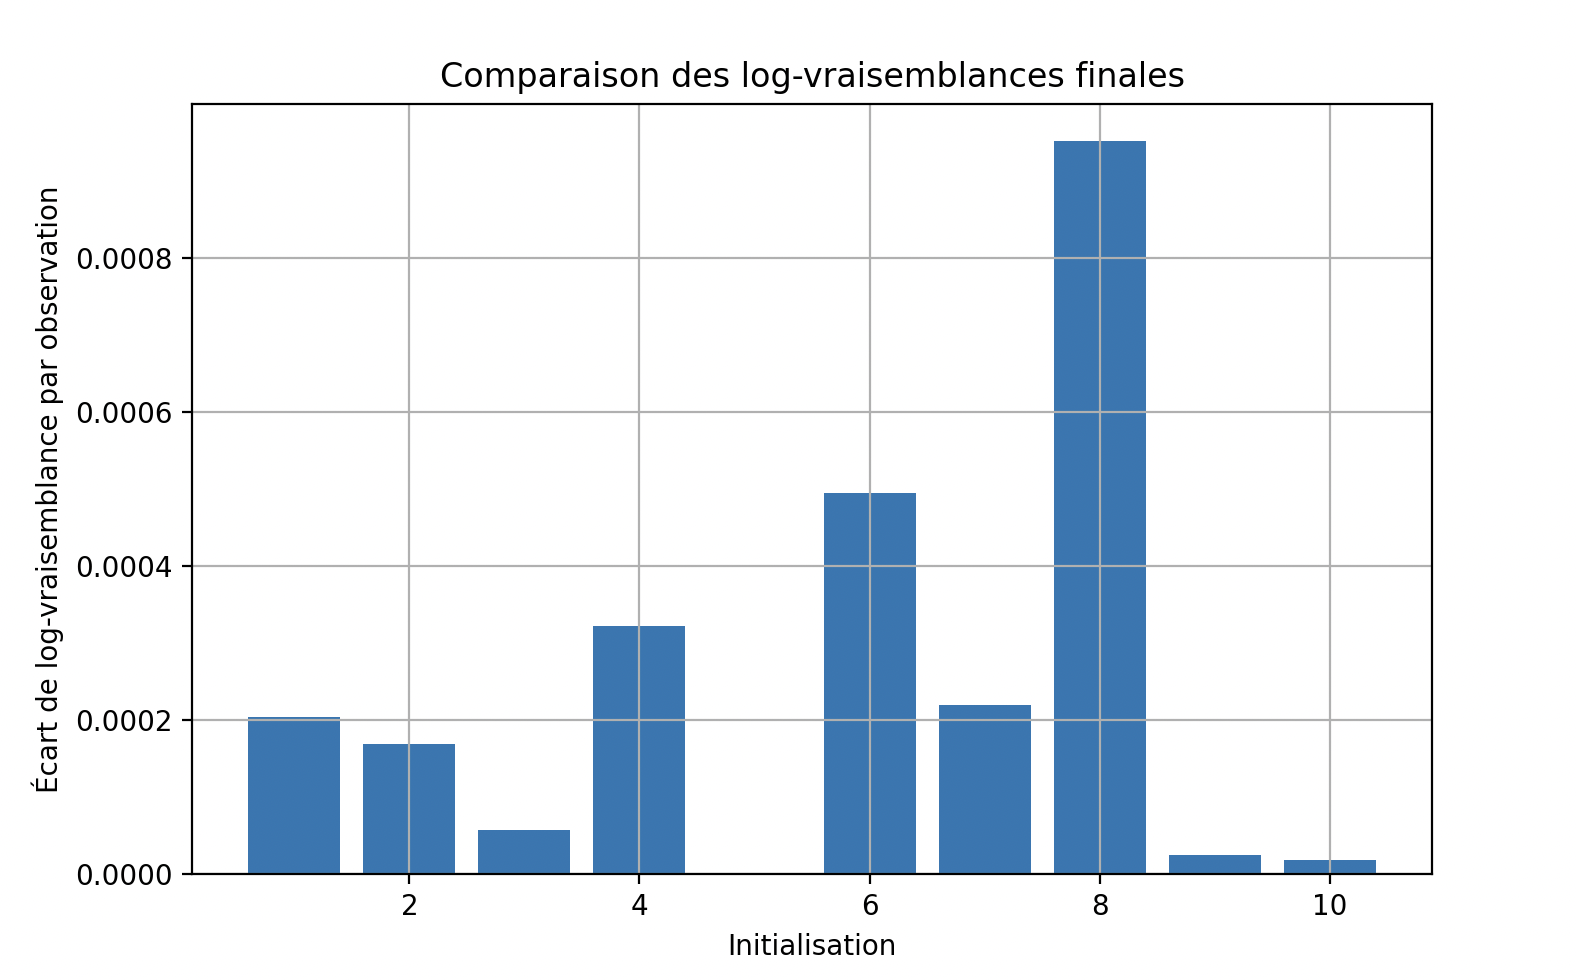
\includegraphics[width=\linewidth]{Test/comparaison_log_vraisemblances.png}

\vspace{0.04cm}

\end{column}

\begin{column}{0.50\textwidth}
\centering
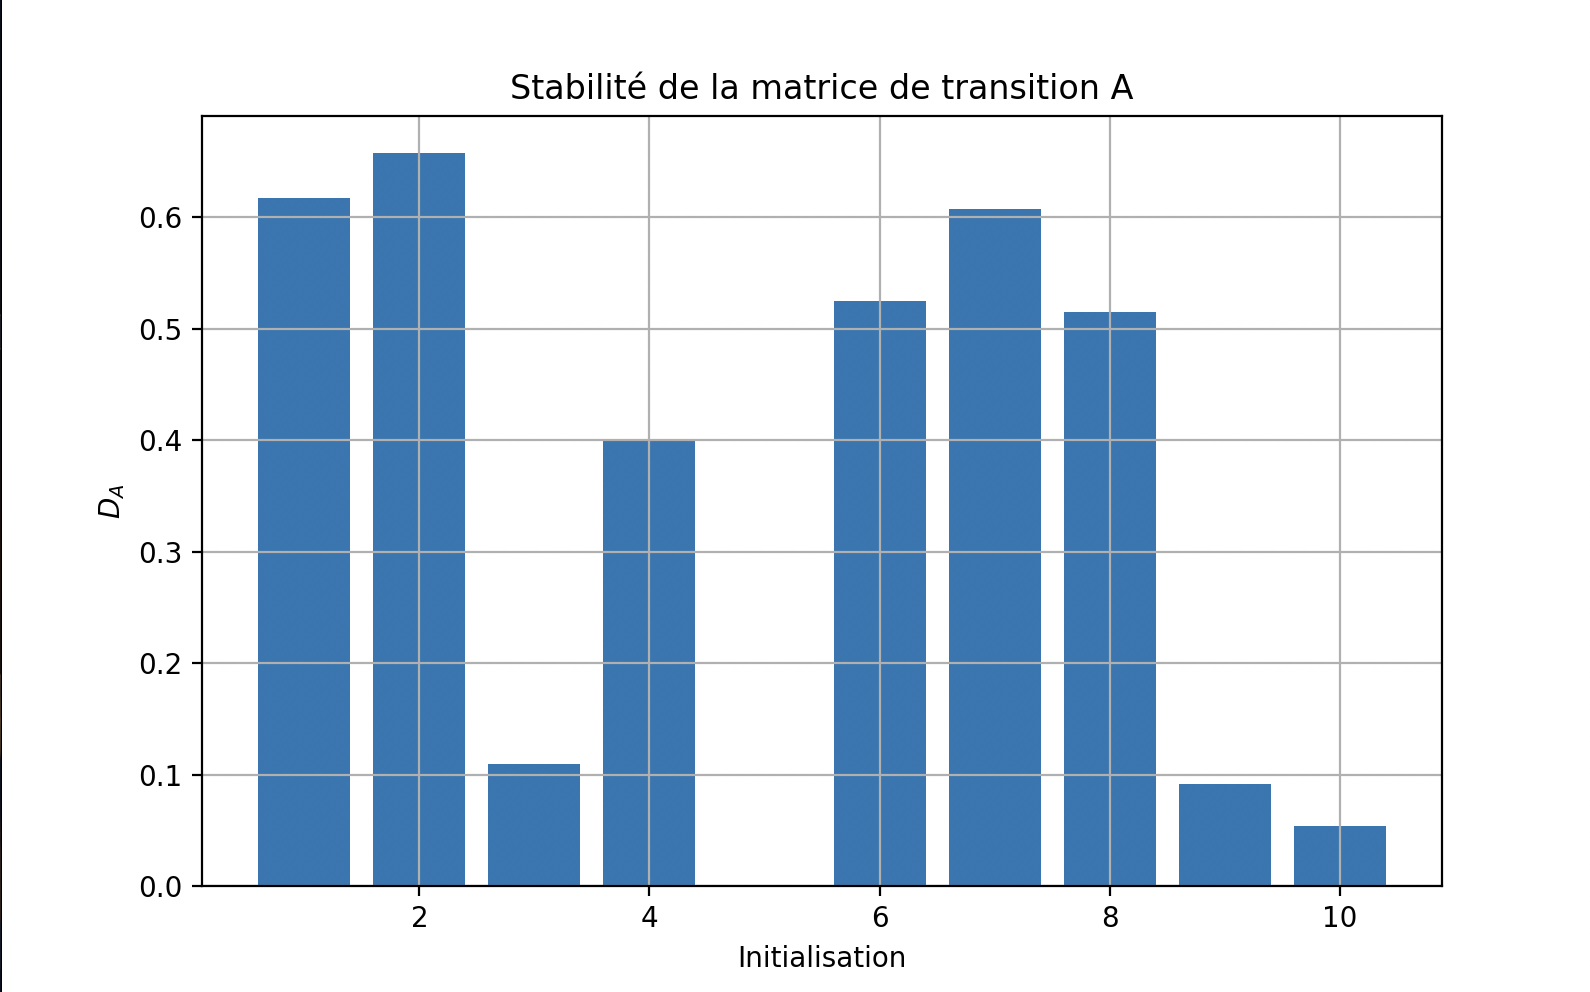
\includegraphics[width=\linewidth]{Test/stabilite_A.png}

\vspace{0.04cm}

\end{column}

\end{columns}

\vspace{0.18cm}

\begin{columns}[T]

\begin{column}{0.50\textwidth}
\centering
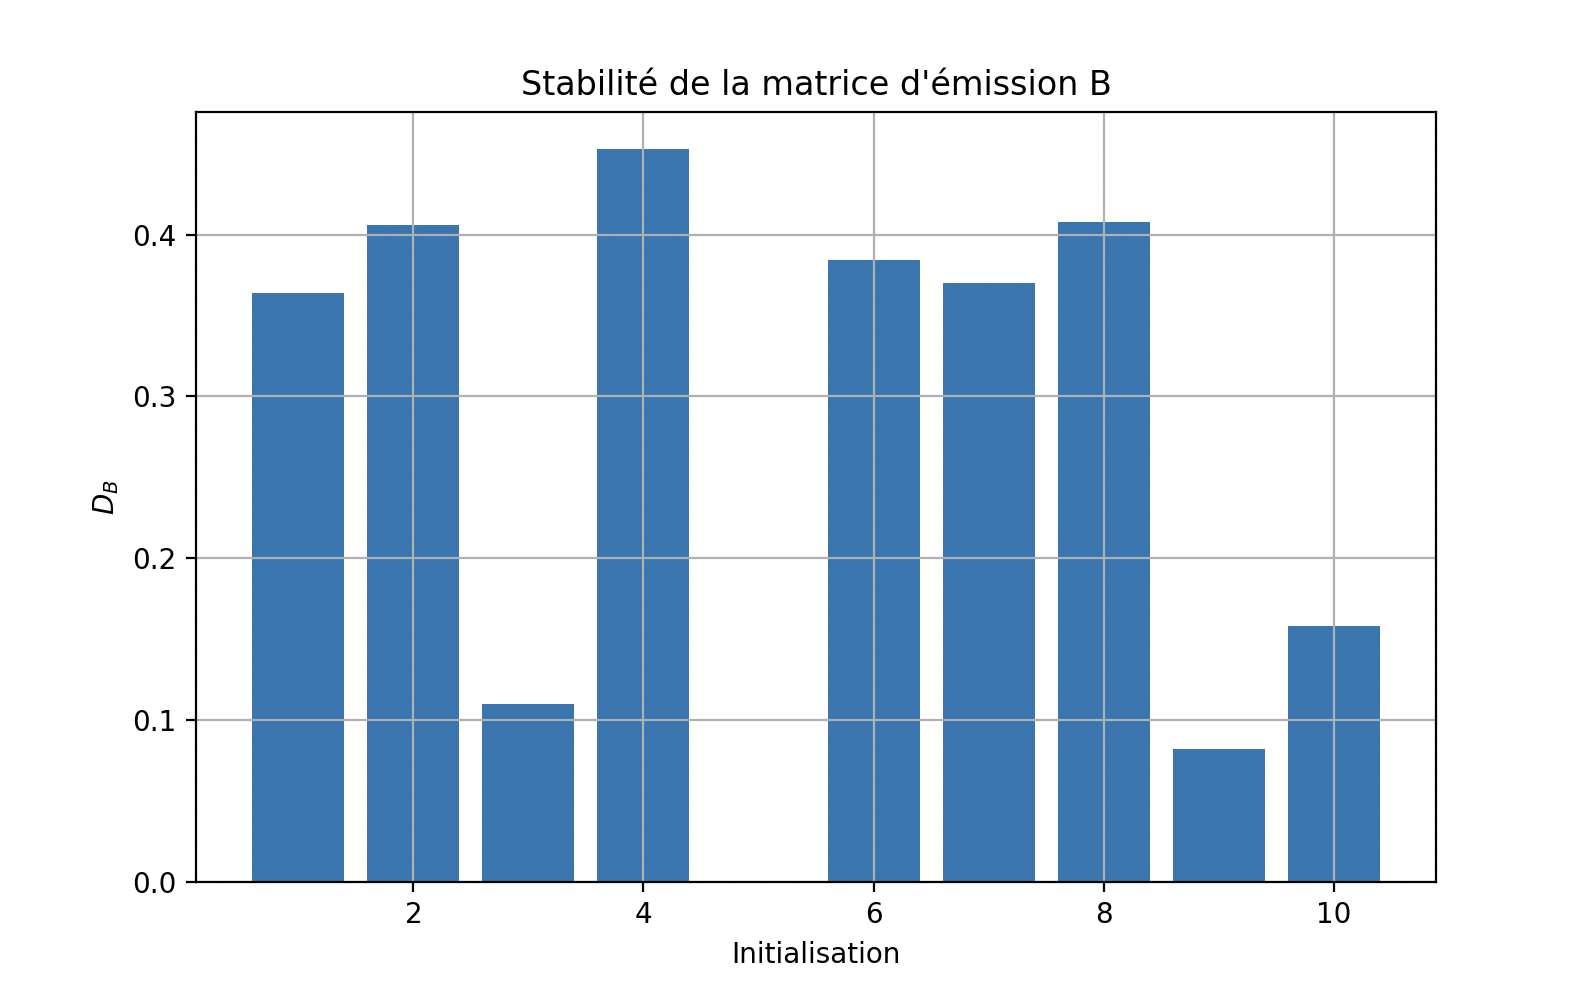
\includegraphics[width=\linewidth]{Test/stabilite_b.png}

\vspace{0.04cm}

\end{column}

\begin{column}{0.50\textwidth}
\centering
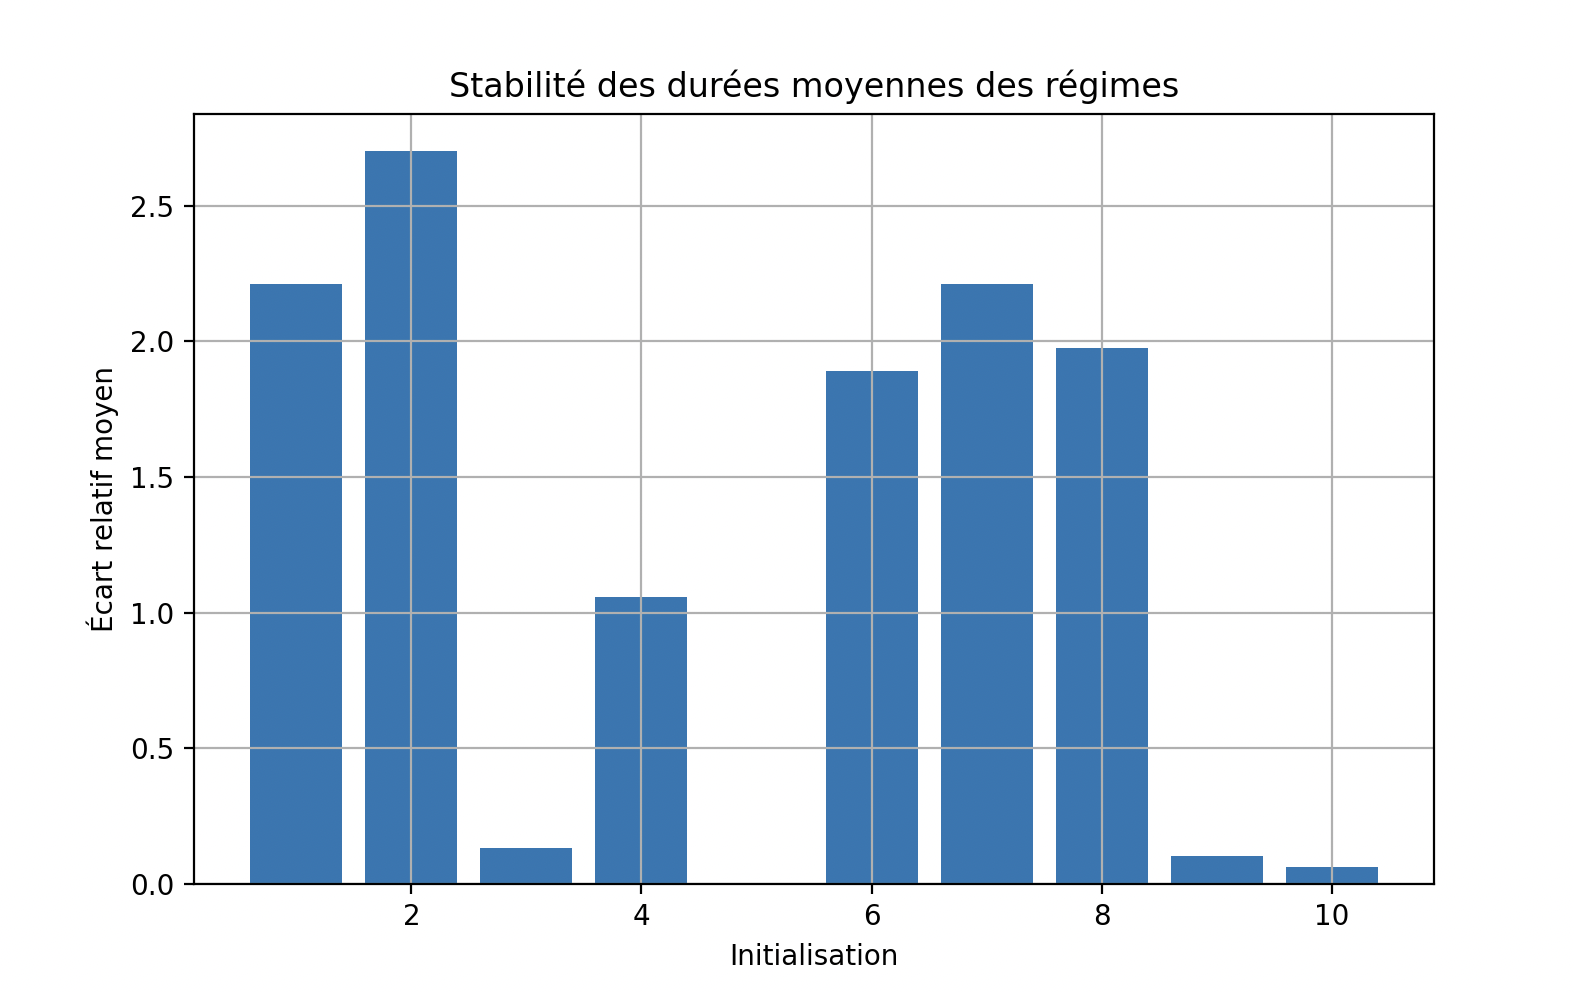
\includegraphics[width=\linewidth]{Test/stabilite_durees.png}

\vspace{0.04cm}

\end{column}

\end{columns}

\end{frame}


\begin{frame}{Application au VIX}

\tiny
\centering

On applique le HMM au VIX en utilisant trois variables observées :
\[
R_t=\log(V_t)-\log(V_{t-1}),
\qquad
\sigma_t^{(5)}=\operatorname{std}(R_{t-4},\dots,R_t),
\qquad
\sigma_t^{(20)}=\operatorname{std}(R_{t-19},\dots,R_t).
\]

\vspace{0.08cm}

Le rendement logarithmique \(R_t\) décrit les variations journalières du VIX, la volatilité courte \(\sigma_t^{(5)}\) capte les mouvements récents, et la volatilité longue \(\sigma_t^{(20)}\) décrit une dynamique plus persistante.

\vspace{0.12cm}

\textbf{Statistiques moyennes obtenues pour les trois régimes}

\vspace{0.05cm}

\resizebox{0.85\linewidth}{!}{
\begin{tabular}{lrrrr}
\toprule
Régime & VIX moyen & \(R_t\) moyen & \(\sigma_t^{(20)}\) moyenne & Nombre d'observations \\
\midrule
Calme & 16.3809 & 0.0007 & 0.0466 & 2364 \\
Intermédiaire & 20.0225 & -0.0021 & 0.0719 & 1751 \\
Crise & 23.6703 & 0.0018 & 0.1134 & 1003 \\
\bottomrule
\end{tabular}
}

\vspace{0.12cm}

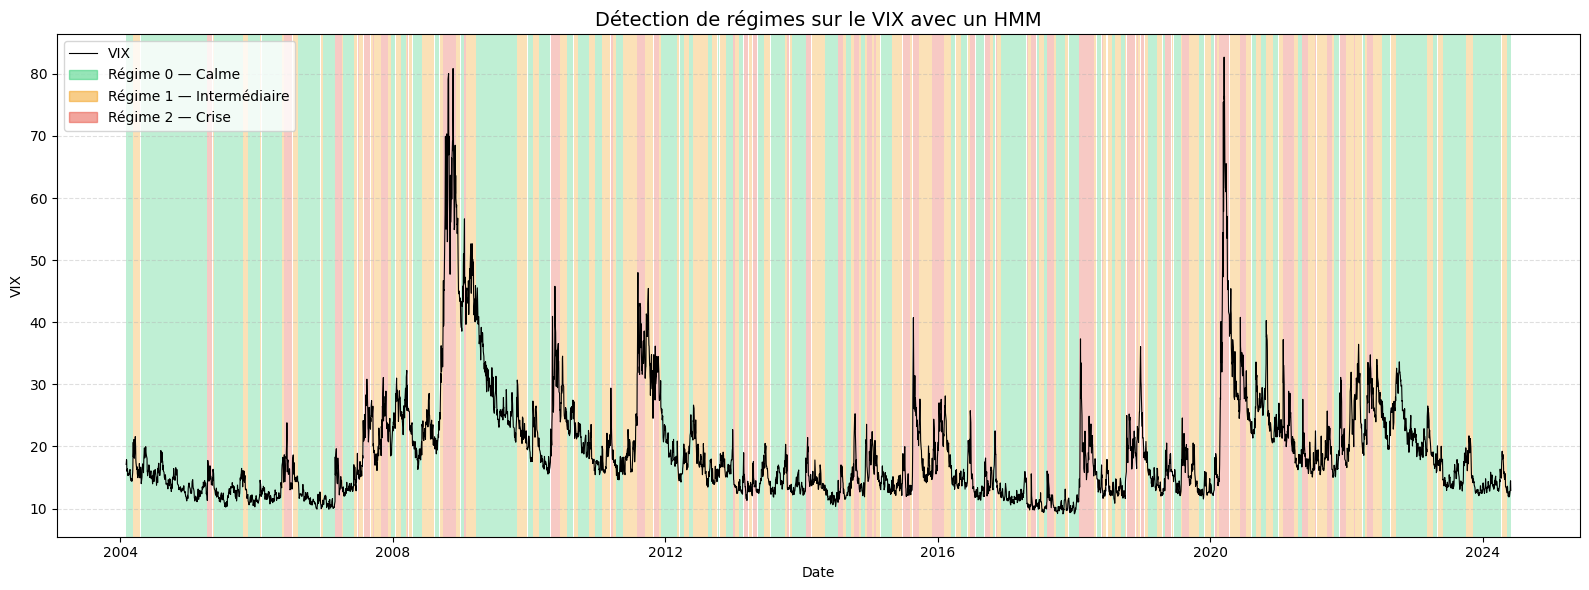
\includegraphics[width=0.85\linewidth]{Figures/regime_detectionVIX.png}

\vspace{0.03cm}


\end{frame}

\begin{frame}{Analyse Baum--Welch sur le VIX}

\tiny
\centering

\begin{columns}[T]

\begin{column}{0.47\textwidth}
\centering
\textbf{Convergence}

\vspace{0.05cm}

\resizebox{\linewidth}{!}{
\begin{tabular}{lr}
\toprule
Critère & Valeur \\
\midrule
Nombre d'observations \(T\) & 5118 \\
Meilleure initialisation & 10 \\
Nombre d'itérations & 36 \\
Log-vraisemblance finale & -14300.087178 \\
Log-vraisemblance moyenne & -2.794077 \\
Gain final / observation & \(9.728857\times 10^{-11}\) \\
Gain relatif final & \(3.481714\times 10^{-11}\) \\
Baisses détectées & 0 \\
\bottomrule
\end{tabular}
}
\end{column}

\begin{column}{0.53\textwidth}
\centering
\textbf{Comparaison des initialisations}

\vspace{0.05cm}

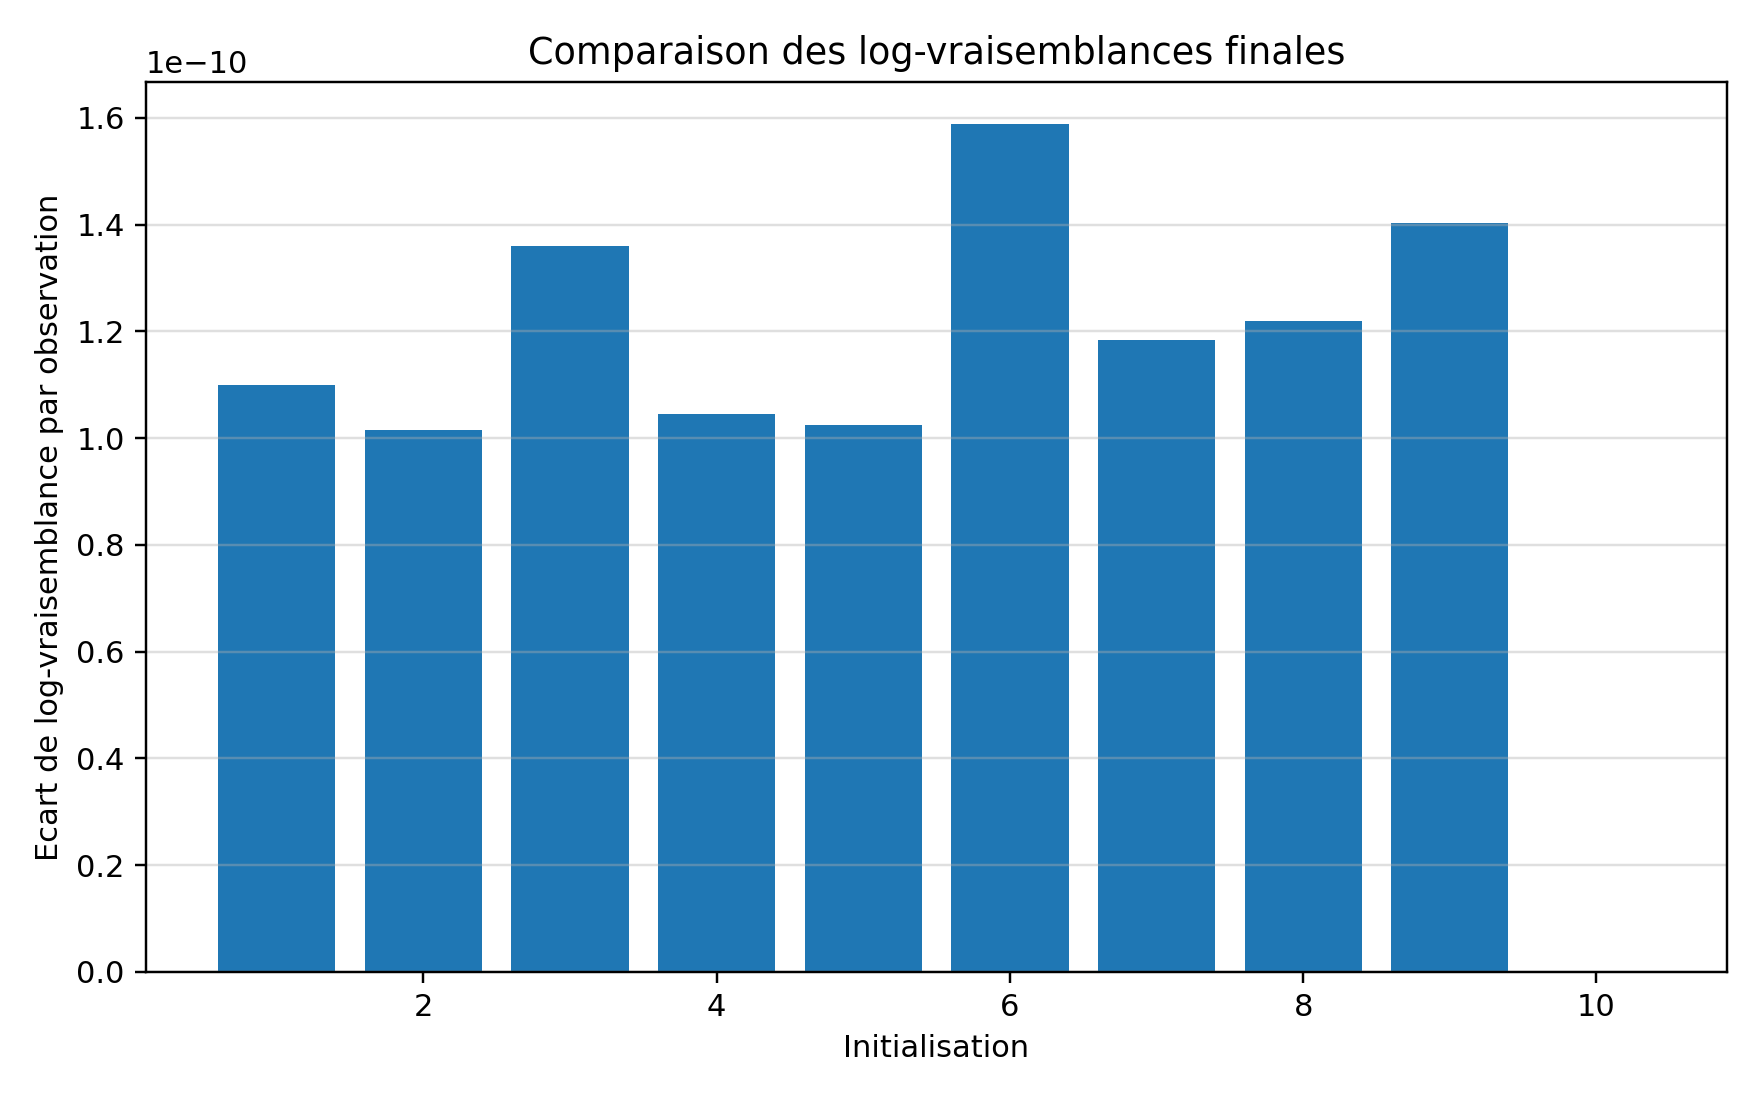
\includegraphics[width=\linewidth]{Test/comparaison_log_vraisemblances_vix.png}

\vspace{0.03cm}

\end{column}

\end{columns}

\vspace{0.2cm}

\textbf{Validation hors échantillon}

\vspace{0.05cm}

\resizebox{0.70\linewidth}{!}{
\begin{tabular}{lrrr}
\toprule
Segment & \(T\) & Log-vraisemblance & NLPD \\
\midrule
Apprentissage & 4094 & -11536.441391 & 2.817890 \\
Test conditionnel & 1024 & -2774.008272 & 2.708992 \\
Test indépendant & 1024 & -2782.320895 & 2.717110 \\
\bottomrule
\end{tabular}
}

\end{frame}




\end{document}
